\documentclass{standalone}

\usepackage{pgfplots,tikz,amsmath}
\begin{document}
        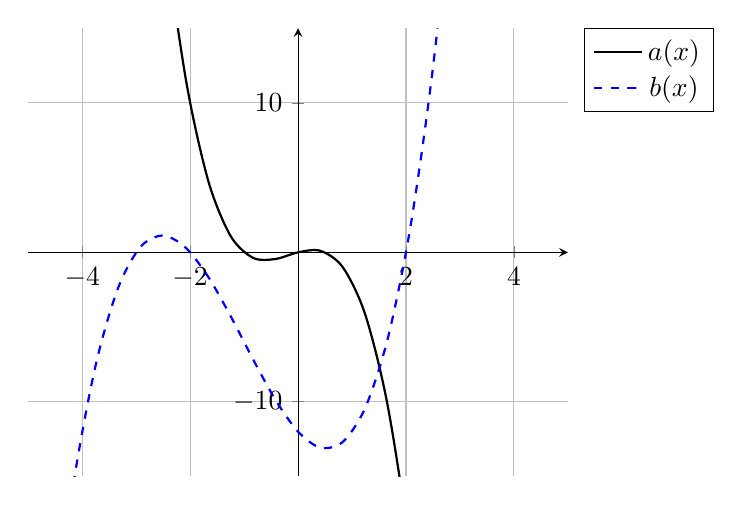
\begin{tikzpicture}
            \begin{axis}[axis lines=center, xmin=-5, xmax=5, ymin=-15, ymax=15, grid,
                legend pos=outer north east]
                \addplot[thick, black, smooth] {-2*x^3-x^2+x};
                \addlegendentry{$a(x)$};
                \addplot[thick, blue, smooth, dashed] {x^3+3*x^2-4*x-12};
                \addlegendentry{$b(x)$};
            \end{axis}
        \end{tikzpicture}
        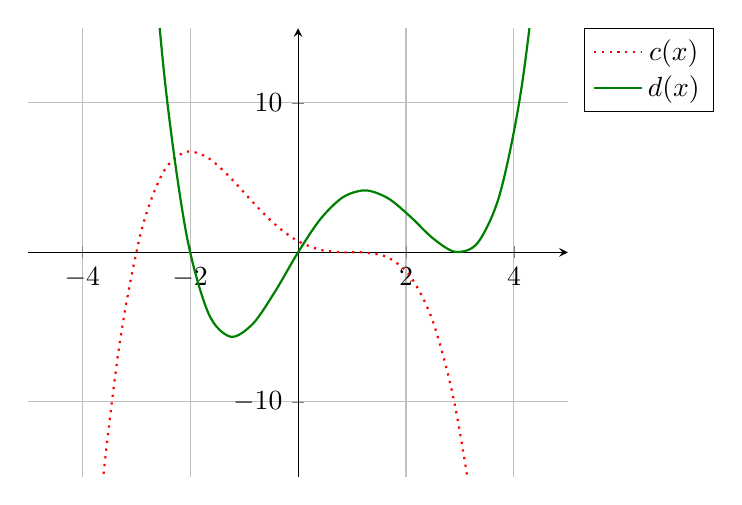
\begin{tikzpicture}
            \begin{axis}[axis lines=center, xmin=-5, xmax=5, ymin=-15, ymax=15, grid,
                legend pos=outer north east]
                \addplot[thick, red, smooth, dotted] {-0.25*(x-1)^3*(x+3)};
                \addlegendentry{$c(x)$};
                \addplot[thick, green!50!black, smooth]
                {(1/3)*x*(x+2)*(x-3)^2};
                \addlegendentry{$d(x)$};
            \end{axis}
        \end{tikzpicture}
\end{document}
